\documentclass[11pt]{report}



\usepackage{wrapfig, graphicx}
\usepackage[total={5.9in,8.86in},top=1.2in, includefoot]{geometry}
\usepackage[font={small},labelfont=bf, justification=raggedright]{caption}
\usepackage{subfig}
\newcommand{\credit}[1]{\textit{(Photo: #1)}}

\begin{document}



\begin{titlepage}
 \begin{center}

\textsc{\large University of Toronto}\\[1.5cm]
\textsc{\normalsize AER201, January 2010}\\[0.5cm]

% Title

{ \huge \bfseries Helical Cone Deployment Machine}\\[0.4cm]

% and supervisor
\begin{minipage}{0.4\textwidth}
\begin{flushleft} \large
\emph{Author:}\\
Ahil Ganesh (997998992)\\
Sebastian Kosch (997241024)\\
Karl Qin (997235123)\\
\end{flushleft}
\end{minipage}
\begin{minipage}{0.4\textwidth}
\begin{flushright} \large
\emph{Supervisor:} \\
Dr. Reza Emami
\end{flushright}
\end{minipage}

\vfill

% Bottom of the page
{\large \today}

\end{center}
\end{titlepage}

\chapter{Executive Summary}
Blabla. This is our machine.

\chapter{Introduction}

\section{Statement of Need}

We {\textit really} need these, because traffic workers die all the time.

\section{Goals and Objectives}

We hope to build a proof-of-concept machine that shows how coil-based deployment machines are not only ridiculously simple, but also ridiculously cheap. In fact, they're so simple and cheap that even the poorest community can build one.

We want to be able to perform the task in less than a minute, hopefully in less than 30 seconds. We want it to be easily usable, quickly loadable, and do fucking well in the competition.

\section{Background Research}

Allegedly invented by a New Yorker in 1914,\footnote{Several websites report this fact. We could not locate a primary source.} traffic cones have proven helpful in redirecting vehicles. However, deploying cones manually on busy highways is a great security risk for road workers. The British Highway Agency, for example, reported 17 fatal accidents involving highway workers from 2000 to 2005 \cite{HTMA-Casualties}. Automatic cone deployment has been recognized as a way to reduce casualties and increase efficiency, and several different approaches are being marketed.

\subsection{Existing Designs}

\begin{figure}
  \centering
  \subfloat[Autocone]{\label{fig:gull}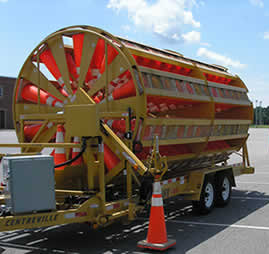
\includegraphics[width=0.45\textwidth]{autocone}}\hspace{20pt}                
  \subfloat[TRAF-tech ACM]{\label{fig:tiger}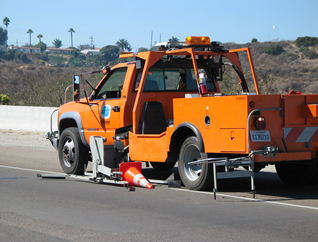
\includegraphics[width=0.45\textwidth]{traftech}}
   \caption{Existing designs \credit{http://www.innovativequip.com/, http://www.traftech.net/}}
  \label{fig:animals}
\end{figure}

\subsubsection{Autocone}
The Autocone 130 is a large trailer that stores up to 130 traffic cones. It uses a hydraulic system both to deploy the cones and to pick up cones standing or lying on the road. The cones are stored in a revolving framework. Within the framework, the cones are moved to the deployment arm by means of a chain conveyor system \cite{HowItsMade-Autocone}. While the compactness of the revolving frame is convincing, the capacity is far higher than that required in this project. For this prototype, designing an intricate miniature hydraulic arm is thus not justifiable.

\subsubsection{TRAF-tech ACT/M Series}
TRAF-tech commercialized the cone deployment system initially developed by the California Department of Transportation. Two different implementations are available: one uses rails to deploy the cones, the other a hydraulic arm. Both rely on belt systems to move the individual cones from the stack to the deployment mechanism. Like Autocone, TRAF-tech offers systems with a comparatively high cone capacity. Conveyor belts, however, are difficult to build reliably,\footnote{as has been confirmed by past AER201 students.} and may not be of much help with the more flexible toy cones at hand.


\subsection{Possible solutions for the given RFP}

Ahil: There are many different solutions, like belts and notches and conveyor belts, alien fingers trying to pry the bent motherfuckers apart, and amazing, godlike coils.

\chapter{Technical Body}

\section{Statement of Work}
\subsection{Mechanical Components}

There are some sweet-ass pieces in this machine. First, the coils. 2 Dollars each, but kicking more ass than an entire fleet of Klingon Cone Deployment Spaceships ever could.

\subsection{Functional Description}

The thing goes, twists the coil one rotation everytime, thereby dropping a cone.

\subsection{Evaluation Plan}
\subsubsection{Process evaluation}
Every week, we'll make sure we're on time.
\subsubsection{Product evaluation}
Gotta be awesome. Duh.

\section{Schedule}
Bar chart, bar chart, bar chart.

\section{Budget}
We need billions, my son.

\chapter{Conclusion}


%\bibliography{


%}

\end{document}
